\documentclass[brazilian,11pt]{beamer}

\graphicspath{{Figuras/}{Figuras internet/}{../Figuras/}{../Figuras internet/}{nepo/img/}{../nepo/img/}}
\usepackage[brazilian,provide=*]{babel}
\usepackage{booktabs}
\usepackage{lmodern}
\usepackage{graphicx}
\usepackage{grffile}
% Figuras ilustrativas (pasta Figuras internet)
\newcommand{\figinternet}[2][width=\linewidth]{%
  \includegraphics[#1,keepaspectratio]{{Figuras internet}/#2}%
}
% Painel: figura com altura fixa + legenda (evita corte na grade 2x2)
\newcommand{\figpainel}[3][0.21\textheight]{%
  \begin{minipage}[c]{\linewidth}%
    \centering
    \figinternet[height=#1]{#2}\\[0.25em]
    {\scriptsize #3}%
  \end{minipage}%
}
\usepackage{amsmath}
\usepackage{amssymb}
\usepackage{ragged2e}
\usepackage{etoolbox}
\apptocmd{\frame}{}{\justifying}{}
\apptocmd{\itemize}{\justifying}{}{}
\apptocmd{\enumerate}{\justifying}{}{}
\addtobeamertemplate{block begin}{}{\justifying}
\addtobeamertemplate{alertblock begin}{}{\justifying}

\usetheme{Boadilla}
\useinnertheme{circles}
% miniframes estoura a largura com muitas seções/frames (overfull hbox ~130pt)
\useoutertheme{default}
\setbeamertemplate{navigation symbols}{}

\setbeamersize{text margin left=0.9cm, text margin right=0.9cm}
\setbeamerfont{block title}{size=\small}
\setbeamerfont{block body}{size=\small}
\setbeamerfont{alertblock title}{size=\small}
\setbeamerfont{alertblock body}{size=\small}
\setbeamerfont{caption}{size=\scriptsize}
\setbeamertemplate{caption}[numbered]

\definecolor{primaryColor}{RGB}{20,45,105}
\definecolor{secondaryColor}{RGB}{0,100,160}
\setbeamercolor{structure}{fg=primaryColor}
\setbeamercolor{palette primary}{bg=primaryColor, fg=white}
\setbeamercolor{palette secondary}{bg=secondaryColor, fg=white}
\setbeamercolor{title}{bg=primaryColor, fg=white}
\setbeamercolor{headline}{bg=secondaryColor, fg=white}
\setbeamercolor{section in head/foot}{bg=primaryColor, fg=white}
\setbeamercolor{subsection in head/foot}{bg=secondaryColor, fg=white}
\setbeamercolor{author in head/foot}{bg=primaryColor, fg=white}
\setbeamercolor{title in head/foot}{bg=secondaryColor, fg=white}
\setbeamercolor{date in head/foot}{bg=primaryColor, fg=white}
\setbeamercolor{page number in head/foot}{bg=primaryColor, fg=white}

\setbeamertemplate{footline}{%
  \leavevmode%
  \hbox{%
    \begin{beamercolorbox}[
      wd=0.42\paperwidth,ht=2.4ex,dp=1ex,leftskip=0.8em,rightskip=0.3em
    ]{author in head/foot}%
      \usebeamerfont{author in head/foot}\insertshortauthor
    \end{beamercolorbox}%
    \begin{beamercolorbox}[
      wd=0.43\paperwidth,ht=2.4ex,dp=1ex,center
    ]{title in head/foot}%
      \usebeamerfont{title in head/foot}\insertshorttitle
    \end{beamercolorbox}%
    \begin{beamercolorbox}[
      wd=0.15\paperwidth,ht=2.4ex,dp=1ex,rightskip=0.8em
    ]{date in head/foot}%
      \usebeamerfont{date in head/foot}\insertframenumber/\inserttotalframenumber
    \end{beamercolorbox}%
  }%
}

\title[Bagging e formas 3D]{Using Bagging to improve clustering methods in the context of three-dimensional shapes}
\subtitle[Nascimento et al., 2024]{Autores: Inácio Nascimento, Raydonal Ospina, Getúlio Amorim \\ --- \textit{Advances in Data Analysis and Classification}}
\author[C. Araújo \& M. Oliveira]{Caio Araújo \& Marina Oliveira}
\institute[UFPE]{Universidade Federal de Pernambuco (UFPE)\\Programa de Pós-Graduação em Estatística}
\date{\today}

\begin{document}

\begin{frame}[plain]
    \begin{center}
        
\includegraphics[width=0.1\linewidth]{Logo-ufpe-2-2 (1).jpg}
    \end{center}
    \vspace{-0.3cm}
    \titlepage
\end{frame}

\begin{frame}[shrink=15]
    \frametitle{Sumário}
    {\footnotesize\tableofcontents[hidesubsections]}
\end{frame}

\section[Intro]{Introdução e Motivação}

\begin{frame}[t]
    \frametitle{O Problema}
    \framesubtitle{Agrupamento de formas geométricas em 3D}

    \vspace{-0.1cm}
    \begin{columns}[T,onlytextwidth]
        \column{0.57\textwidth}
        \begin{block}{Contexto motivador}
            \small
            Classificar objetos pela \textbf{forma} --- estrutura geométrica após remover escala e posição --- é central em paleontologia, medicina e engenharia. O tamanho sozinho raramente basta para separar grupos.
        \end{block}
        \column{0.41\textwidth}
        \figpainel[0.30\textheight]{fóssil.png}{Morfologia de fósseis: agrupamento por forma, não por escala.}
    \end{columns}
\end{frame}

\begin{frame}[t]
    \frametitle{Aplicações da análise de formas}
    \framesubtitle{Aplicações em morfometria e análise de formas}

    \vspace{-0.2cm}
    \begin{columns}[T,onlytextwidth]
        \column{0.49\textwidth}
        \figpainel[0.175\textheight]{cerebro.png}{Medicina / neurociência (ex.: córtex, RM)}
        \vspace{0.25em}
        \figpainel[0.175\textheight]{coração.png}{Medicina: morfologia cardíaca}
        \column{0.49\textwidth}
        \figpainel[0.175\textheight]{motor.png}{Engenharia: controle de qualidade 3D}
        \vspace{0.25em}
        \figpainel[0.175\textheight]{abelhas.png}{Biologia: morfologia e classificação de espécies}
    \end{columns}
\end{frame}

\begin{frame}[t]
    \frametitle{Lacuna na literatura e objetivos}
    \framesubtitle{Contribuição de Nascimento et al.\ (2024)}

    \vspace{-0.1cm}
    \begin{block}{Lacuna na literatura}
        \footnotesize
        \begin{itemize}
            \item Poucos métodos de agrupamento adaptados a formas 3D
            \item Passar de 2D para 3D não é ``só mais uma dimensão'' (espaço estratificado)
            \item Vinué et al.\ (2014): k-means e k-means podado para 3D
        \end{itemize}
    \end{block}
    \vspace{0.15em}
    \begin{block}{Objetivo}
        \footnotesize
        \begin{enumerate}
            \item Adaptar \textbf{k-means}, \textbf{CLARANS} e \textbf{Hill Climbing} ao espaço de formas 3D
            \item Aplicar \textbf{Bagging} (BagClust1) para melhorar estabilidade e acurácia
            \item Avaliar com simulação e dados reais (RI e FMI)
        \end{enumerate}
    \end{block}
\end{frame}

\begin{frame}[t]
    \frametitle{Desafio central}
    \framesubtitle{Por que formas 3D exigem métodos específicos}

    \vspace{-0.1cm}
    \begin{columns}[T,onlytextwidth]
        \column{0.52\textwidth}
        \begin{alertblock}{Desafio central}
            \small
            Formas 3D vivem em \textbf{espaços não euclidianos} (estratificados, com singularidades). Não basta usar distância euclidiana e média aritmética usuais.
        \end{alertblock}
        \vspace{0.2em}
        \small
        \begin{itemize}
            \item Remover efeitos de \textbf{localização}, \textbf{escala} e \textbf{rotação}
            \item Comparar objetos com distâncias adequadas ao espaço de formas (Dryden \& Mardia, 2016; Nascimento et al., 2024)
        \end{itemize}
        \column{0.45\textwidth}
        \figpainel[0.34\textheight]{Ilustração_analogia_intuitiva.png}{Variedade suave (2D) vs.\ singularidades (3D).}
    \end{columns}
\end{frame}

\section[Formas]{Background: Análise Estatística de Formas}

\begin{frame}[shrink=8]
    \frametitle{Fundamentos da análise de formas}
    \framesubtitle{Configurações e espaço de formas (Dryden \& Mardia, 2016)}

    \begin{block}{Definição --- Kendall (1977)}
        \textbf{Forma}: informação geométrica que permanece ao remover efeitos de \textbf{localização}, \textbf{escala} e \textbf{rotação}.
    \end{block}

    \begin{itemize}
        \item \textbf{Marcos (\textit{landmarks})}: conjunto finito de pontos na silhueta do objeto
        \item \textbf{Configuração}: matriz $X \in \mathbb{R}^{k \times m}$, com $k$ marcos e $m=3$ coordenadas cartesianas
        \item \textbf{Espaço de configurações}: todas as coordenadas possíveis dos marcos
    \end{itemize}

    \begin{block}{Definição 1 --- Espaço de formas}
        Conjunto de \textbf{classes de equivalência} das matrizes $X$ sob transformações de similaridade euclidiana (translação, rotação e escala). Admite estrutura de variedade riemanniana; para $m \geq 3$ torna-se \textbf{espaço estratificado} (singularidades).
    \end{block}
\end{frame}

\begin{frame}[t]
    \frametitle{Por que não usar similaridade euclidiana?}
    \framesubtitle{Parâmetros de nuisance e invariância geométrica}

    \vspace{-0.15cm}
    \begin{columns}[T,onlytextwidth]
        \column{0.51\textwidth}
        \footnotesize
        A matriz $X$ depende de \textbf{localização}, \textbf{escala} e \textbf{rotação}. Duas capturas do mesmo objeto podem ter coordenadas muito diferentes (ex.: mesma cadeira em posições distintas).
        \begin{itemize}
            \setlength{\itemsep}{0.15em}
            \item Comparar $X$ diretamente confunde forma com posição e orientação
            \item Pipeline: Helmert $\rightarrow$ pré-forma $Z$ $\rightarrow$ classe $[Z]$
        \end{itemize}
        \column{0.47\textwidth}
        \figpainel[0.34\textheight]{O problema das similaridades euclidianas.png}{Mesma forma, coordenadas distintas.}
    \end{columns}
\end{frame}

\begin{frame}[shrink=10]
    \frametitle{Pré-forma e remoção de efeitos}
    \framesubtitle{Coordenadas de Kendall e matriz de Helmert}

    \small
    A matriz $X$ não é invariante a similaridades euclidianas. Remove-se translação multiplicando $X$ pela submatriz de Helmert $H$ (Dryden \& Mardia, 2016, p.~49).

    \begin{block}{Pré-forma (Nascimento et al., 2024, eq.~1)}
        \begin{equation}
            Z = \frac{HX}{\|HX\|}, \qquad
            \|HX\|^2 = \mathrm{tr}\bigl((HX)^{\mathsf T}(HX)\bigr)
        \end{equation}
        $Z$ é a \textbf{pré-forma}: efeitos de escala removidos; \textbf{rotação permanece}.
    \end{block}

    \begin{block}{Definição 2 --- Espaço de pré-formas $\mathcal{S}_m^k$}
        \[
            \mathcal{S}_m^k = \left\{ Z = \frac{HX}{\|HX\|} : X \in \mathbb{R}^{k \times m} \right\}
        \]
        Para $m=3$, $\mathcal{S}_m^k$ é hiperesfera unitária em $\mathbb{R}^{(k-1)m}$ (subvariedade riemanniana).
    \end{block}
\end{frame}

\begin{frame}[shrink=8]
    \frametitle{Forma e análise de Procrustes}
    \framesubtitle{Definição 3 e comparação de objetos}

    \begin{block}{Definição 3 --- Forma de uma configuração}
        \begin{equation}
            [Z] = \{ Z\Gamma : \Gamma \in SO(m) \}
        \end{equation}
        $\Gamma$ é matriz de rotação; $SO(m)$ é o grupo ortogonal especial. O espaço de formas $\Sigma_m^k$ é quociente de $\mathcal{S}_m^k$ sob rotações.
    \end{block}

    \textbf{Procrustes}: alinha formas por transformações rígidas, minimizando distância entre pontos homólogos. Duas configurações $X_1$, $X_2$ têm pré-formas $Z_1$, $Z_2$.

    \vspace{0.2em}
    \footnotesize\textit{Observação:} em 3D o espaço $\Sigma_m^k$ não é variedade suave; na prática assume-se variação restrita, longe das singularidades.
\end{frame}

\begin{frame}[shrink=12]
    \frametitle{Distâncias e forma média}
    \framesubtitle{Definições 4--6 (Nascimento et al., 2024)}

    \small
    \begin{block}{Definição 4 --- Distância riemanniana $\rho(X_1,X_2)$}
        Menor distância ao longo de \textbf{grande círculo} (sobre rotações) entre $Z_1$ e $Z_2$ em $\mathcal{S}_m^k$.
    \end{block}

    \begin{block}{Definição 5 --- Distância de Procrustes completa}
        \begin{equation}
            d_F(X_1, X_2) = \inf_{\Gamma \in SO(m),\, \beta \in \mathbb{R}_+} \left\| Z_2 - \beta Z_1 \Gamma \right\|, \qquad d_F = \sin(\rho)
        \end{equation}
    \end{block}

    \begin{block}{Definição 6 --- Média de Procrustes (Fréchet)}
        \begin{equation}
            [\hat{\mu}] = \arg\min_{\mu} \sum_{i=1}^{n} d_F^2(X_i, \mu)
        \end{equation}
        Para $m \geq 3$ a média é obtida \textbf{iterativamente} (Algoritmo~1, Dryden \& Mardia, 2016).
    \end{block}
\end{frame}

\section[Algoritmos]{Algoritmos de Agrupamento Adaptados}

\begin{frame}
    \frametitle{Agrupamento de formas tridimensionais}
    \framesubtitle{Notação comum (Nascimento et al., 2024)}

    \begin{block}{Problema}
        Classificar objetos em grupos com base na \textbf{forma}, não nas coordenadas brutas.
    \end{block}

    \begin{itemize}
        \item Conjunto de dados: $\mathcal{X} = \{X_i,\ i = 1,\ldots,n\}$, cada $X_i$ é matriz de configuração ($k \times 3$)
        \item Algoritmos produzem partição $G = (G_r,\ r = 1,\ldots,K)$ com $K$ grupos
        \item Métodos: k-means (Vinué et al., 2014), CLARANS e Hill Climbing (Nascimento et al., 2024)
    \end{itemize}

    \vspace{0.3em}
    \small Todos usam distâncias do espaço de formas (Definições~4--6), não distância euclidiana em $\mathbb{R}^{k \times m}$.
\end{frame}

\begin{frame}[shrink=8]
    \frametitle{3.1 K-means para formas 3D}
    \framesubtitle{Algoritmo de Lloyd adaptado (Vinué et al., 2014)}

    \small
    A distância euclidiana do k-means clássico é substituída pela \textbf{distância riemanniana} $\rho$ (Definição~4). O centroide $\mu_r$ de cada grupo é a \textbf{forma média de Procrustes} (Algoritmo~1).

    \begin{block}{Critério WSS (Nascimento et al., 2024, eq.~4)}
        \begin{equation}
            W = \sum_{r=1}^{K} \sum_{i \in G_r} \mathrm{Dist}^2(X_i, \mu_r)
        \end{equation}
        $G_r$ contém as observações do grupo $r$; $\mathrm{Dist}$ é a distância riemanniana; $\mu_r$ é obtido por Algoritmo~1.
    \end{block}

    \textbf{Algoritmo 2} (passos): (i) atribuir cada $X_i$ ao centroide mais próximo; (ii) recalcular $\mu_r$; repetir até convergência.

    \begin{itemize}
        \item Partição inicial aleatória $\Rightarrow$ ótimo local; recomenda-se várias inicializações
        \item Sensível a \textit{outliers}: centroides são médias, não objetos do conjunto
    \end{itemize}
\end{frame}

\begin{frame}[shrink=5]
    \frametitle{3.2 CLARANS para formas 3D}
    \framesubtitle{Extensão do PAM com busca aleatorizada (Ng \& Han, 2002)}

    \begin{block}{Medoides (PAM)}
        Representante $m_r$ de $G_r$ é um \textbf{ponto real} do grupo com menor dissimilaridade média aos demais --- mais robusto que a média do k-means.
    \end{block}

    \begin{itemize}
        \item Grafo $G_{n,K}$: nós = conjuntos de $K$ medoides; cada nó define uma partição distinta
        \item Vizinhos diferem por \textbf{um único} medoide; cada nó tem até $K(n-K)$ vizinhos
        \item \textbf{Custo} de um nó: dissimilaridade total entre cada objeto e o medoide do seu grupo
        \item CLARANS busca nó de custo mínimo via amostragem de vizinhos (PAM em subconjunto)
    \end{itemize}

    Parâmetros: \texttt{numlocal} (buscas locais), \texttt{maxneighbor} (máx.\ vizinhos examinados). Adaptação 3D: Algoritmo~3 (Nascimento et al., 2024), com distâncias riemannianas.
\end{frame}

\begin{frame}[shrink=8]
    \frametitle{3.3 Hill Climbing para formas 3D}
    \framesubtitle{Friedman \& Rubin (1967); critério TD}

    \small
    Busca local: reestrutura a partição e mantém a nova configuração somente se o critério melhorar (minimização $\Rightarrow$ ``descida de colina'').

    \begin{block}{Dissimilaridade total (Nascimento et al., 2024, eq.~5)}
        \begin{equation}
            TD = \sum_{r=1}^{K} \sum_{i \in G_r} d(X_i, m_r)
        \end{equation}
        $m_r$ é o \textbf{medoide} de $G_r$; $d$ é distância no espaço de formas. Quanto \textbf{menor} $TD$, melhor o agrupamento.
    \end{block}

    \textbf{Algoritmo 4} (Nascimento et al., 2024): atualização dos medoides nos passos de reatribuição. Pode ficar em ótimo local; o Bagging visa reduzir essa instabilidade.
\end{frame}

\section[Bagging]{A Proposta: Bagging}

\begin{frame}
    \frametitle{Bagging: conceito e motivação}
    \framesubtitle{Bootstrap Aggregating e clustering ensemble}

    \begin{block}{Conceito}
        \textbf{Bagging} (\textit{Bootstrap Aggregating}, Breiman, 1996) é uma técnica de \textbf{ensemble}: combina várias execuções do mesmo algoritmo para obter um resultado mais estável.
    \end{block}

    \begin{itemize}
        \item Procedimento \textbf{BagClust1} (Dudoit \& Fridlyand, 2003; Nascimento et al., 2024)
        \item Motivação: algoritmos de partição são instáveis --- pequenas mudanças nos dados alteram o agrupamento
        \item $B = 100$ réplicas bootstrap (originalmente Dudoit usava $B=20$)
    \end{itemize}
\end{frame}

\begin{frame}
    \frametitle{Procedimento BagClust1}
    \framesubtitle{Etapas do ensemble por votação}

    \begin{enumerate}
        \item Gerar $B$ amostras \textbf{bootstrap} (com reposição) do conjunto de formas 3D
        \item Aplicar k-means, CLARANS ou Hill Climbing em \textbf{cada} amostra
        \item Alinhar rótulos entre partições (permutações)
        \item \textbf{Consenso por votação}: para cada objeto, atribuir o rótulo mais frequente entre as $B$ execuções
        \item Em caso de empate: escolha aleatória
    \end{enumerate}

    \begin{alertblock}{Vantagens esperadas}
        \begin{itemize}
            \item Reduz \textbf{variância} e flutuações aleatórias
            \item Mitiga ótimos locais e efeito de \textit{outliers}
            \item Especialmente útil quando CLARANS usa \texttt{maxneighbor} pequeno
        \end{itemize}
    \end{alertblock}
\end{frame}

\section[Simulação]{Estudo de Simulação}

\begin{frame}[shrink=5]
    \frametitle{Avaliação numérica}
    \framesubtitle{Comparação dos métodos com e sem Bagging}

    \begin{itemize}
        \item Comparar k-means, CLARANS e Hill Climbing \textbf{com} e \textbf{sem} Bagging ($B=100$, BagClust1)
        \item Dissimilaridade: \textbf{distância riemanniana} (Definição~4); implementação em \textbf{R} (pacotes de formas 3D)
        \item $K=2$ grupos conhecidos \textit{a priori} (particionamento); $K$ desconhecido $\Rightarrow$ hierárquico (Everitt et al., 2001)
    \end{itemize}

    \begin{block}{Parâmetros dos algoritmos (Nascimento et al., 2024)}
        \footnotesize
        \begin{itemize}
            \item \textbf{K-means}: critério de parada em (4) com tolerância $10^{-4}$; 10 inicializações e 10 passos por inicialização (melhor partição)
            \item \textbf{CLARANS}: \texttt{numlocal}$=2$; \texttt{maxneighbor}$=0{,}0125 \cdot K(N-K)$
            \item \textbf{Hill Climbing}: encerra ao atingir tamanho máximo do laço de busca
        \end{itemize}
    \end{block}
\end{frame}

\begin{frame}[shrink=10]
    \frametitle{Geração dos dados simulados}
    \framesubtitle{Seguindo Vinué et al.\ (2014) --- espaço de marcos}

    \small
    Duas figuras geométricas fixas: \textbf{cubo} (grupo~1) e \textbf{paralelepípedo} (grupo~2), cada uma com $k=8$ marcos ($m=3$).

    \begin{itemize}
        \item Para cada grupo $i=1,2$: simular $n_i$ objetos a partir de
        \[
            \mathbf{X} \sim \mathcal{N}_{3k}\bigl(\boldsymbol{\mu}_i,\, \boldsymbol{\Sigma}_i\bigr),
        \]
        onde $\boldsymbol{\mu}_i$ é o vetor médio ($3k$) da forma-base (cubo ou paralelepípedo) e $\boldsymbol{\Sigma}_i$ é $3k \times 3k$.
        \item Orientação arbitrária das formas-base; depois aplica-se \textbf{rotação} em torno do eixo $z$ com ângulo aleatório da função \texttt{rvm} (\textit{CircStats})
        \item Coordenadas simuladas são transformadas em \textbf{matrizes de configuração} $k \times 3$
    \end{itemize}

    \begin{block}{Distribuição von Mises (rotação)}
        \[
            f(\theta;\mu,\kappa) = \frac{1}{2\pi I_0(\kappa)} \exp\{\kappa\cos(\theta-\mu)\}
        \]
        $I_0(\kappa)$: Bessel modificada; $\mu$ direção média; $\kappa$ concentração (Best \& Fisher, 1979).
    \end{block}
\end{frame}

\begin{frame}[shrink=12]
    \frametitle{Cenários de dispersão}
    \framesubtitle{Isotropia e anisotropia (Nascimento et al., 2024)}

    \small
    Em todos os cenários: $\sigma_1=\sigma_2 \in \{3,\,6,\,9\}$ (baixa, média e alta dispersão).

    \begin{block}{Isotropia --- mesma variabilidade em todas as direções}
        \[
            \boldsymbol{\Sigma}_i = \sigma_i^2 \, \mathbf{I}_{3k \times 3k}, \qquad i=1,2
        \]
        Os marcos têm variabilidade aproximadamente igual em todas as coordenadas.
    \end{block}

    \begin{block}{Anisotropia --- variabilidade direcional}
        \[
            \boldsymbol{\Sigma}_i = \frac{\sigma_i^2}{2\gamma}\Bigl(
            \mathbf{1}_k\mathbf{1}_k^{\mathsf T}
            + (\gamma-1)\mathbf{I}_k \otimes \mathbf{1}_m\mathbf{1}_m^{\mathsf T}
            + (\gamma-1)\mathbf{I}_{m \times m}\Bigr), \quad \gamma = 4,\; m=3
        \]
        Produto de Kronecker: dispersões diferem entre direções dos marcos.
    \end{block}
\end{frame}

\begin{frame}[shrink=8]
    \frametitle{Desenho experimental e validação}
    \framesubtitle{Monte Carlo, índices e testes}

    \begin{columns}[T]
        \column{0.52\textwidth}
        \begin{block}{Amostra e réplicas}
            \begin{itemize}
                \item Cada conjunto: $N=100$ objetos ($n_1=n_2=50$ cubos / paralelepípedos)
                \item \textbf{50 réplicas} de Monte Carlo por cenário (variabilidade vs.\ custo computacional)
                \item Em cada réplica: várias partições iniciais até convergência; guarda-se a \textbf{melhor} partição (menor $W$ ou $TD$)
                \item Bagging: $B=100$ amostras bootstrap + votação (Dudoit \& Fridlyand, 2003)
            \end{itemize}
        \end{block}

        \column{0.46\textwidth}
        \begin{block}{Métricas e inferência}
            \begin{itemize}
                \item \textbf{RI} (Rand) e \textbf{FMI} (Fowlkes--Mallows) $\in [0,1]$; 1 = concordância perfeita com grupos verdadeiros
                \item Resultados agregados (Nascimento et al., 2024, Tabelas~1--6): média $\bar{x}$ e desvio-padrão \textit{sd} sobre 50 réplicas
                \item \textbf{Wilcoxon pareado} ($\alpha=5\%$): $H_0$ sem diferença; $H_1$ método \textbf{sem} Bagging pior que \textbf{com} Bagging
            \end{itemize}
        \end{block}
    \end{columns}

    \vspace{0.2em}
    \footnotesize\textit{Observação:} na simulação compara-se a distribuição das 50 réplicas (Wilcoxon). Nos \textbf{dados reais}, emprega-se o \textbf{ganho relativo} em RI e FMI (Nascimento et al., 2024).
\end{frame}

\begin{frame}
    \frametitle{Formas Simuladas}
    \framesubtitle{Cubo e paralelepípedo com 8 marcos}
    \centering
    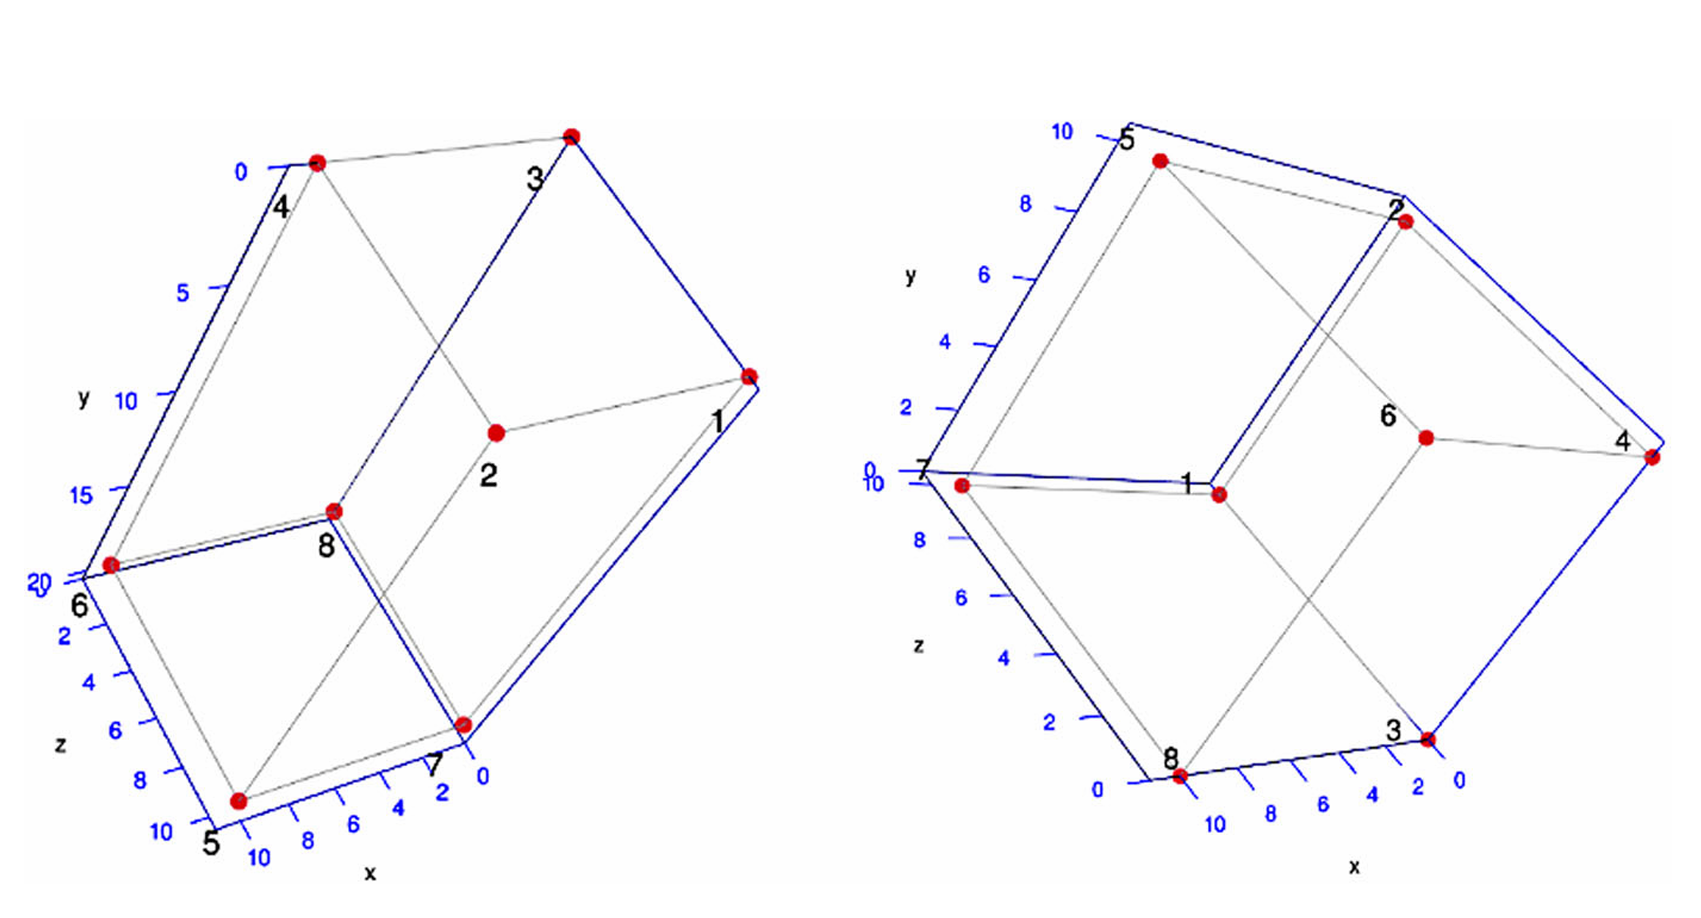
\includegraphics[height=0.38\textheight,keepaspectratio]{fig01_cubo_paralelepipedo.png}
    \hspace{0.02\textwidth}
    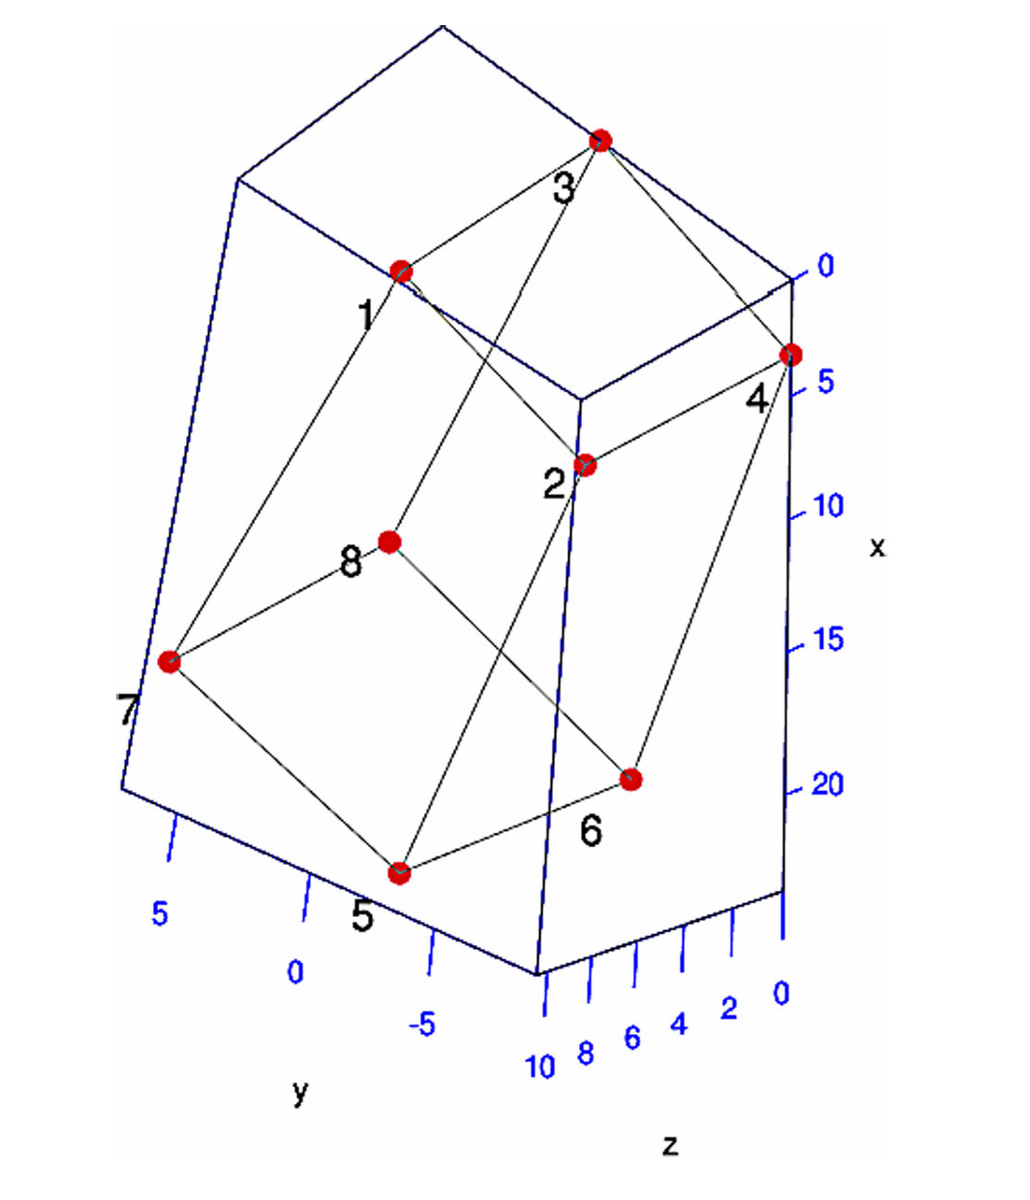
\includegraphics[height=0.38\textheight,keepaspectratio]{fig02_paralelepipedo_rotacionado.png}
    \vfill
    {\scriptsize Figuras 1 e 2: Cubo e paralelepípedo formados por 8 marcos, e paralelepípedo rotacionado aleatoriamente.}
\end{frame}

\section[Resultados]{Resultados das Simulações}

\begin{frame}[shrink=8]
    \frametitle{Efeito do Bagging na simulação}
    \framesubtitle{Síntese dos resultados (Nascimento et al., 2024)}

    \begin{columns}[T]
        \column{0.48\textwidth}
        \begin{block}{Baixa dispersão ($\sigma = 3$)}
            \small Pouco ganho com Bagging --- métodos já são ótimos.
        \end{block}
        \begin{block}{Média/alta ($\sigma = 6$, $9$)}
            \small CLARANS e Hill Climbing melhoram (Wilcoxon, 5\%).
        \end{block}
        \column{0.48\textwidth}
        \begin{alertblock}{k-means}
            \small Ganhos limitados; melhorias pontuais em alta dispersão (FMI).
        \end{alertblock}
        \begin{itemize}
            \item \small CLARANS e Hill Climbing: maiores beneficiários
            \item \small RI e FMI caem quando a dispersão aumenta
        \end{itemize}
    \end{columns}
\end{frame}

% --- Isotropia ---
\begin{frame}
    \frametitle{Resultados: Isotropia}
    \vfill
    \centering
    \begin{table}
        \centering
        \caption{\justifying Resultados para os algoritmos k-means e k-means Bagging aplicados a dados simulados de cubos e paralelepípedos representados por $k = 8$ marcos, sob isotropia.}
        \resizebox{\linewidth}{!}{%
            \begin{tabular}{lcccccccccc}
            \toprule
            Isotropic variation & \multicolumn{5}{c}{Rand index} & \multicolumn{5}{c}{Fowlkes-mallows index} \\
            \cmidrule(lr){2-6} \cmidrule(lr){7-11}
            & \multicolumn{2}{c}{Without bagging} & \multicolumn{2}{c}{B=100} & $p$ value & \multicolumn{2}{c}{Without bagging} & \multicolumn{2}{c}{B=100} & $p$ value \\
            \cmidrule(lr){2-3} \cmidrule(lr){4-5} \cmidrule(lr){7-8} \cmidrule(lr){9-10}
            & $\bar{x}$ & sd & $\bar{x}$ & sd & & $\bar{x}$ & sd & $\bar{x}$ & sd & \\
            \midrule
            $\sigma_1 = \sigma_2 = 3$ & 1 & 0 & 1 & 0 & 1.0000 & 1 & 0 & 1 & 0 & 1.0000 \\
            $\sigma_1 = \sigma_2 = 6$ & 0.9175 & 0.0320 & 0.9148 & 0.0309 & 0.9218 & 0.9169 & 0.0321 & 0.9139 & 0.0309 & 0.9290 \\
            $\sigma_1 = \sigma_2 = 9$ & 0.6656 & 0.0667 & 0.6720 & 0.0646 & 0.0788 & 0.6657 & 0.0664 & 0.6744 & 0.0633 & 0.0254 \\
            \bottomrule
            \end{tabular}%
        }
    \end{table}
    \vfill
\end{frame}

\begin{frame}
    \frametitle{Resultados: Isotropia}
    \vfill
    \centering
    \begin{table}
        \centering
        \caption{\justifying Resultados para os algoritmos CLARANS e CLARANS Bagging aplicados a dados simulados de cubos e paralelepípedos representados por $k = 8$ marcos, sob isotropia.}
        \resizebox{\linewidth}{!}{%
            \begin{tabular}{lcccccccccc}
            \toprule
            Isotropic variation & \multicolumn{5}{c}{Rand index} & \multicolumn{5}{c}{Fowlkes-mallows index} \\
            \cmidrule(lr){2-6} \cmidrule(lr){7-11}
            & \multicolumn{2}{c}{Without bagging} & \multicolumn{2}{c}{B=100} & $p$ value & \multicolumn{2}{c}{Without bagging} & \multicolumn{2}{c}{B=100} & $p$ value \\
            \cmidrule(lr){2-3} \cmidrule(lr){4-5} \cmidrule(lr){7-8} \cmidrule(lr){9-10}
            & $\bar{x}$ & sd & $\bar{x}$ & sd & & $\bar{x}$ & sd & $\bar{x}$ & sd & \\
            \midrule
            $\sigma_1 = \sigma_2 = 3$ & 0.9948 & 0.0118 & 1 & 0 & 0.0017 & 0.9948 & 0.0119 & 0.9996 & 0.0028 & 0.0030 \\
            $\sigma_1 = \sigma_2 = 6$ & 0.7027 & 0.0926 & 0.7937 & 0.0645 & $<0.0001$ & 0.7093 & 0.0885 & 0.7979 & 0.0594 & $<0.0001$ \\
            $\sigma_1 = \sigma_2 = 9$ & 0.5322 & 0.0361 & 0.5499 & 0.0452 & 0.0002 & 0.5396 & 0.0397 & 0.5666 & 0.0530 & $<0.0001$ \\
            \bottomrule
            \end{tabular}%
        }
    \end{table}
    \vfill
\end{frame}


\begin{frame}
    \frametitle{Resultados: Isotropia}
    \vfill
    \centering
    \begin{table}
        \centering
        \caption{\justifying Resultados para os algoritmos Hill Climbing e Hill Climbing Bagging aplicados a dados simulados de cubos e paralelepípedos representados por $k = 8$ marcos, sob isotropia.}
        \resizebox{\linewidth}{!}{%
            \begin{tabular}{lcccccccccc}
            \toprule
            Isotropic variation & \multicolumn{5}{c}{Rand index} & \multicolumn{5}{c}{Fowlkes-mallows index} \\
            \cmidrule(lr){2-6} \cmidrule(lr){7-11}
            & \multicolumn{2}{c}{Without bagging} & \multicolumn{2}{c}{B=100} & $p$ value & \multicolumn{2}{c}{Without bagging} & \multicolumn{2}{c}{B=100} & $p$ value \\
            \cmidrule(lr){2-3} \cmidrule(lr){4-5} \cmidrule(lr){7-8} \cmidrule(lr){9-10}
            & $\bar{x}$ & sd & $\bar{x}$ & sd & & $\bar{x}$ & sd & $\bar{x}$ & sd & \\
            \midrule
            $\sigma_1 = \sigma_2 = 3$ & 0.9980 & 0.0061 & 1 & 0 & 0.0184 & 0.9979 & 0.0061 & 1 & 0 & 0.0184 \\
            $\sigma_1 = \sigma_2 = 6$ & 0.7365 & 0.1044 & 0.8617 & 0.0559 & $<0.0001$ & 0.7432 & 0.0973 & 0.8611 & 0.0545 & $<0.0001$ \\
            $\sigma_1 = \sigma_2 = 9$ & 0.5316 & 0.0359 & 0.5741 & 0.0585 & $<0.0001$ & 0.5452 & 0.0392 & 0.5960 & 0.00607 & $<0.0001$ \\
            \bottomrule
            \end{tabular}%
        }
    \end{table}
    \vfill
\end{frame}

\begin{frame}
    \frametitle{Isotropia: Violin Plots}
    \framesubtitle{Diferenças pareadas (Bagging $-$ método original)}
    \centering
    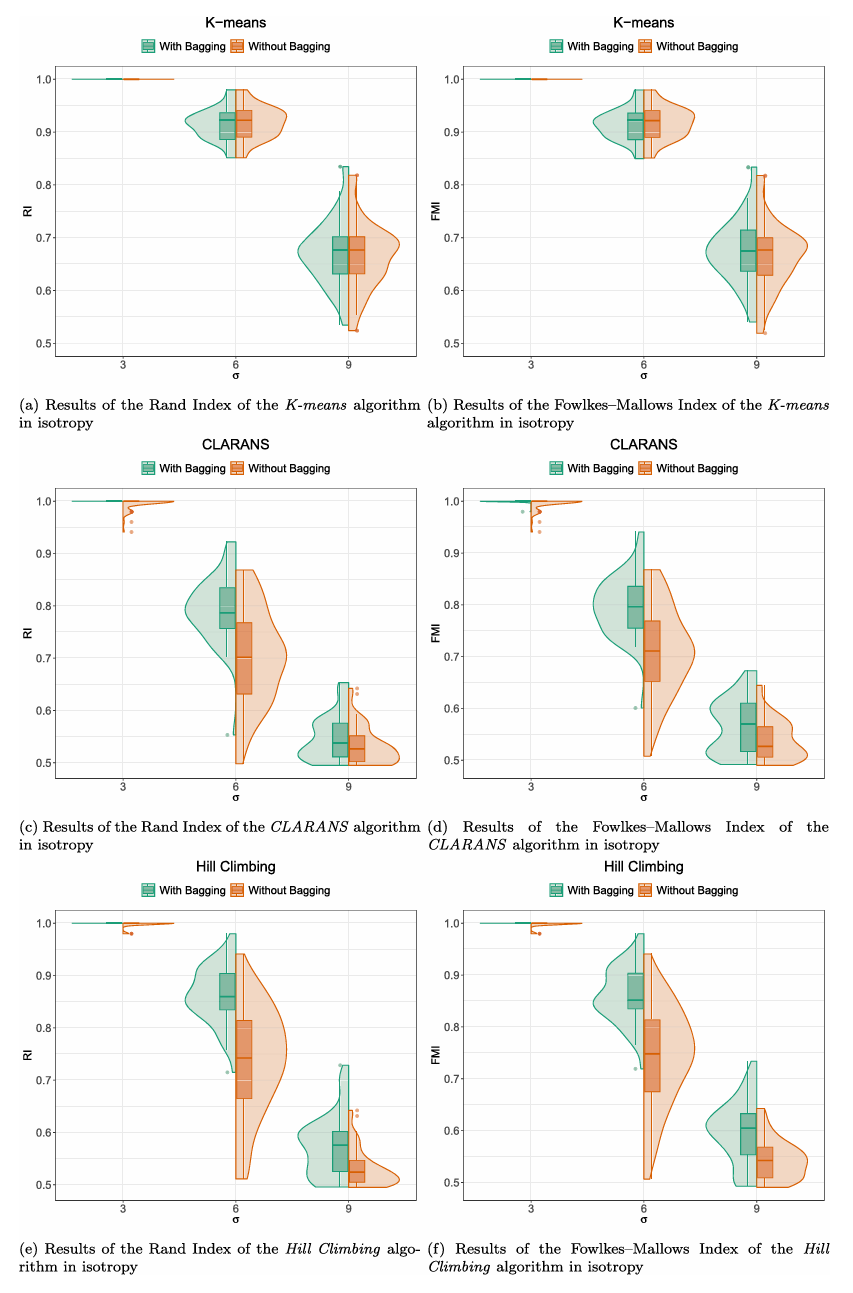
\includegraphics[height=0.66\textheight,keepaspectratio]{fig03_violino_isotropia.png}
    \vfill
    {\scriptsize Figura 3: Gráficos de violino pareados comparando o Bagging e o algoritmo original para os dados simulados sob isotropia.}
\end{frame}

% --- Anisotropia ---
\begin{frame}
    \frametitle{Resultados: Anisotropia}
    \vfill
    \centering
    \begin{table}
        \centering
        \caption{\justifying Resultados para os algoritmos k-means e k-means Bagging aplicados a dados simulados de cubos e paralelepípedos representados por $k = 8$ marcos, sob anisotropia.}
        \resizebox{\linewidth}{!}{%
            \begin{tabular}{lcccccccccc}
            \toprule
            Anisotropic variation & \multicolumn{5}{c}{Rand index} & \multicolumn{5}{c}{Fowlkes-mallows index} \\
            \cmidrule(lr){2-6} \cmidrule(lr){7-11}
            & \multicolumn{2}{c}{Without bagging} & \multicolumn{2}{c}{B=100} & $p$ value & \multicolumn{2}{c}{Without bagging} & \multicolumn{2}{c}{B=100} & $p$ value \\
            \cmidrule(lr){2-3} \cmidrule(lr){4-5} \cmidrule(lr){7-8} \cmidrule(lr){9-10}
            & $\bar{x}$ & sd & $\bar{x}$ & sd & & $\bar{x}$ & sd & $\bar{x}$ & sd & \\
            \midrule
            $\sigma_1 = \sigma_2 = 3$ & 1 & 0 & 1 & 0 & 1.0000 & 1 & 0 & 1 & 0 & 1.0000 \\
            $\sigma_1 = \sigma_2 = 6$ & 0.9623 & 0.0275 & 0.9608 & 0.0275 & 0.9812 & 0.9620 & 0.0276 & 0.9600 & 0.0275 & 0.9882 \\
            $\sigma_1 = \sigma_2 = 9$ & 0.7761 & 0.0601 & 0.7745 & 0.0561 & 0.8529 & 0.7761 & 0.0597 & 0.7755 & 0.0542 & 0.6347 \\
            \bottomrule
            \end{tabular}%
        }
    \end{table}
    \vfill
\end{frame}

\begin{frame}
    \frametitle{Resultados: Anisotropia}
    \vfill
    \centering
    \begin{table}
        \centering
        \caption{\justifying Resultados para os algoritmos CLARANS e CLARANS Bagging aplicados a dados simulados de cubos e paralelepípedos representados por $k = 8$ marcos, sob anisotropia.}
        \resizebox{\linewidth}{!}{%
            \begin{tabular}{lcccccccccc}
            \toprule
            Anisotropic variation & \multicolumn{5}{c}{Rand index} & \multicolumn{5}{c}{Fowlkes-mallows index} \\
            \cmidrule(lr){2-6} \cmidrule(lr){7-11}
            & \multicolumn{2}{c}{Without bagging} & \multicolumn{2}{c}{B=100} & $p$ value & \multicolumn{2}{c}{Without bagging} & \multicolumn{2}{c}{B=100} & $p$ value \\
            \cmidrule(lr){2-3} \cmidrule(lr){4-5} \cmidrule(lr){7-8} \cmidrule(lr){9-10}
            & $\bar{x}$ & sd & $\bar{x}$ & sd & & $\bar{x}$ & sd & $\bar{x}$ & sd & \\
            \midrule
            $\sigma_1 = \sigma_2 = 3$ & 0.9992 & 0.0039 & 1 & 0 & 0.1728 & 0.9992 & 0.0040 & 1 & 0 & 0.1728 \\
            $\sigma_1 = \sigma_2 = 6$ & 0.7909 & 0.1004 & 0.8911 & 0.0426 & <0.0001 & 0.7937 & 0.0962 & 0.8933 & 0.0392 & <0.0001 \\
            $\sigma_1 = \sigma_2 = 9$ & 0.5719 & 0.0651 & 0.6179 & 0.0765 & $<0.0001$ & 0.5792 & 0.0665 & 0.6358 & 0.0757 & $<0.0001$ \\
            \bottomrule
            \end{tabular}%
        }
    \end{table}
    \vfill
\end{frame}

\begin{frame}
    \frametitle{Resultados: Anisotropia}
    \vfill
    \centering
    \begin{table}
        \centering
        \caption{\justifying Resultados para os algoritmos Hill Climbing e Hill Climbing Bagging aplicados a dados simulados de cubos e paralelepípedos representados por $k = 8$ marcos, sob anisotropia.}
        \resizebox{\linewidth}{!}{%
            \begin{tabular}{lcccccccccc}
            \toprule
            Anisotropic variation & \multicolumn{5}{c}{Rand index} & \multicolumn{5}{c}{Fowlkes-mallows index} \\
            \cmidrule(lr){2-6} \cmidrule(lr){7-11}
            & \multicolumn{2}{c}{Without bagging} & \multicolumn{2}{c}{B=100} & $p$ value & \multicolumn{2}{c}{Without bagging} & \multicolumn{2}{c}{B=100} & $p$ value \\
            \cmidrule(lr){2-3} \cmidrule(lr){4-5} \cmidrule(lr){7-8} \cmidrule(lr){9-10}
            & $\bar{x}$ & sd & $\bar{x}$ & sd & & $\bar{x}$ & sd & $\bar{x}$ & sd & \\
            \midrule
            $\sigma_1 = \sigma_2 = 3$ & 1 & 0 & 1 & 0 & 1.0000 & 1 & 0 & 1 & 0 & 1.0000 \\
            $\sigma_1 = \sigma_2 = 6$ & 0.8525 & 0.0884 & 0.9358 & 0.0342 & $<0.0001$ & 0.8548 & 0.0833 & 0.9346 & 0.0345 & $<0.0001$ \\
            $\sigma_1 = \sigma_2 = 9$ & 0.5705 & 0.0546 & 0.6596 & 0.0662 & $<0.0001$ & 0.5842 & 0.0511 & 0.6768 & 0.0609 & $<0.0001$ \\
            \bottomrule
            \end{tabular}%
        }
    \end{table}
    \vfill
\end{frame}

\begin{frame}
    \frametitle{Anisotropia: Violin Plots}
    \framesubtitle{Padrão semelhante ao cenário isotrópico}
    \centering
    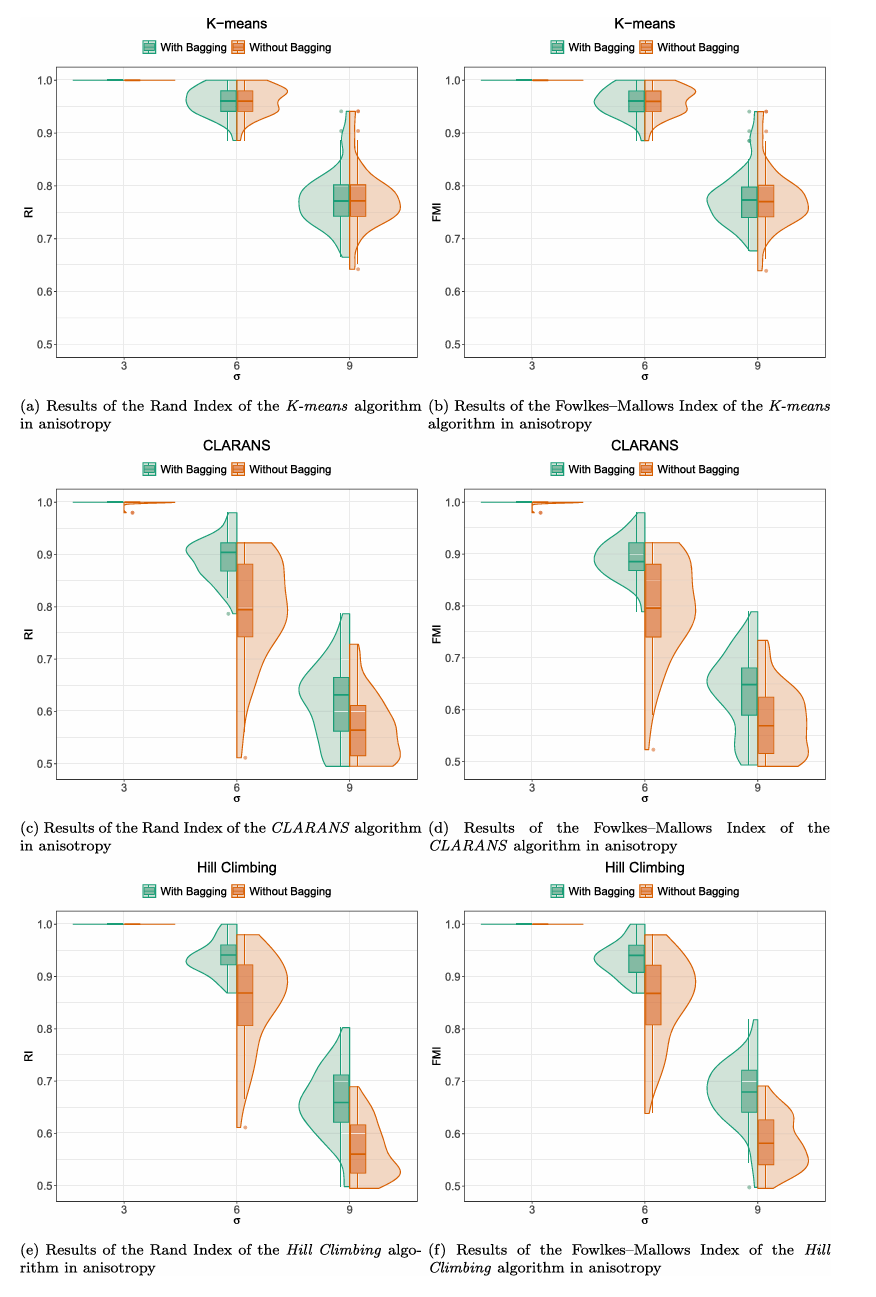
\includegraphics[height=0.66\textheight,keepaspectratio]{fig04_violino_anisotropia.png}
    \vfill
    {\scriptsize Figura 4: Gráficos de violino pareados comparando o Bagging e o algoritmo original para os dados simulados sob anisotropia.}
\end{frame}

\section[Dados reais]{Aplicações em Dados Reais}

\begin{frame}
    \frametitle{Ganho relativo}
    \framesubtitle{Medida de validação nos dados reais (Nascimento et al., 2024)}

    \small
    Para comparar a eficácia dos métodos \textbf{com} e \textbf{sem} Bagging em RI e FMI, Nascimento et al.\ (2024) definem o ganho relativo (\%):

    \begin{equation}
        \text{Ganho relativo}
        = 100 \times
        \frac{\mathrm{VI}_{\mathrm{Bagging}} - \mathrm{VI}}{\mathrm{VI}}
    \end{equation}

    \begin{itemize}
        \item $\mathrm{VI}$: valor do índice de validação (\textbf{Rand} ou \textbf{Fowlkes--Mallows}) \textbf{sem} Bagging
        \item $\mathrm{VI}_{\mathrm{Bagging}}$: valor do mesmo índice \textbf{com} Bagging ($B=100$)
        \item Uma execução por algoritmo; resultados reportados nas Tabelas~7 e~8 (Nascimento et al., 2024)
    \end{itemize}
\end{frame}

\begin{frame}[t]
    \frametitle{Aplicação a dados reais}
    \framesubtitle{Morfometria 3D: validação empírica}

    \begin{columns}[c]
        \column{0.55\textwidth}
        \begin{itemize}
            \item \textbf{Crânios de macacos} ($N=18$, $k=7$): sexo como grupo verdadeiro; conjunto pequeno e bem separado
            \item \textbf{Cérebros humanos} ($N=58$, $k=24$): destros vs.\ canhotos; maior complexidade e ganhos claros com Bagging
            \item Objetos representados por \textbf{marcos anatômicos} em $\mathbb{R}^{k \times 3}$; distância riemanniana em todo o estudo
        \end{itemize}
        \column{0.42\textwidth}
        \figpainel[0.40\textheight]{cerebro.png}{Neuroimagem: contexto das aplicações em morfometria cerebral.}
    \end{columns}
\end{frame}

\begin{frame}[shrink=10]
    \frametitle{Conjunto de dados 1: Crânios de macacos}
    \framesubtitle{\textit{Macaca fascicularis} --- $N=18$, $k=7$ marcos}

    \begin{columns}[c]
        \column{0.5\textwidth}
        \begin{itemize}
            \item $K=2$: 9 machos, 9 fêmeas
            \item Ganhos relativos altos no FMI usando Bagging para CLARANS e Hill Climbing.
        \end{itemize}
        \column{0.5\textwidth}
        \centering
        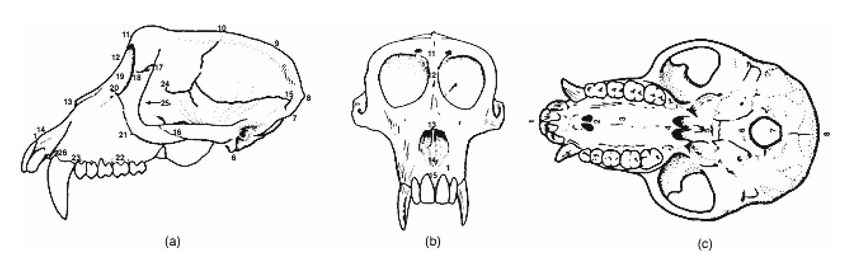
\includegraphics[width=0.8\linewidth,keepaspectratio]{fig05_cranio_macaco.png}
        \par {\scriptsize Figura 5: Representação 3D de um crânio de macaco: (a) lateral; (b) frontal; (c) inferior.}
    \end{columns}
    
    \vspace{0.4cm}
    \centering
    \textbf{Tabela 7} (Nascimento et al., 2024): Resultados para o conjunto \textit{Macaque Skull}.\\[0.05cm]
    {\scriptsize Colunas \textit{relative}: ganho relativo (\%) para RI e FMI.}\\[0.1cm]
    \resizebox{0.95\linewidth}{!}{
        \begin{tabular}{@{}lcccccc@{}}
        \toprule
        Methods & \multicolumn{2}{c}{Rand index} & RI relative & \multicolumn{2}{c}{Fowlkes-mallows index} & FMI relative \\
        \cmidrule(lr){2-3} \cmidrule(lr){5-6}
         & Without bagging & B=100 & gain & Without bagging & B=100 & gain \\
        \midrule
        K-means & 0.4967 & 0.4967 & 0.00\% & 0.6214 & 0.6214 & 0.00\% \\
        CLARANS & 0.5294 & 0.5294 & 0.00\% & 0.5527 & 0.6124 & 10.78\% \\
        Hill Climbing & 0.4771 & 0.4967 & 4.11\% & 0.5025 & 0.6124 & 21.86\% \\
        \bottomrule
        \end{tabular}
    }
\end{frame}

\begin{frame}
    \frametitle{Macacos: Agrupamento nas PCs}
    \framesubtitle{Visualização em componentes principais}
    \centering
    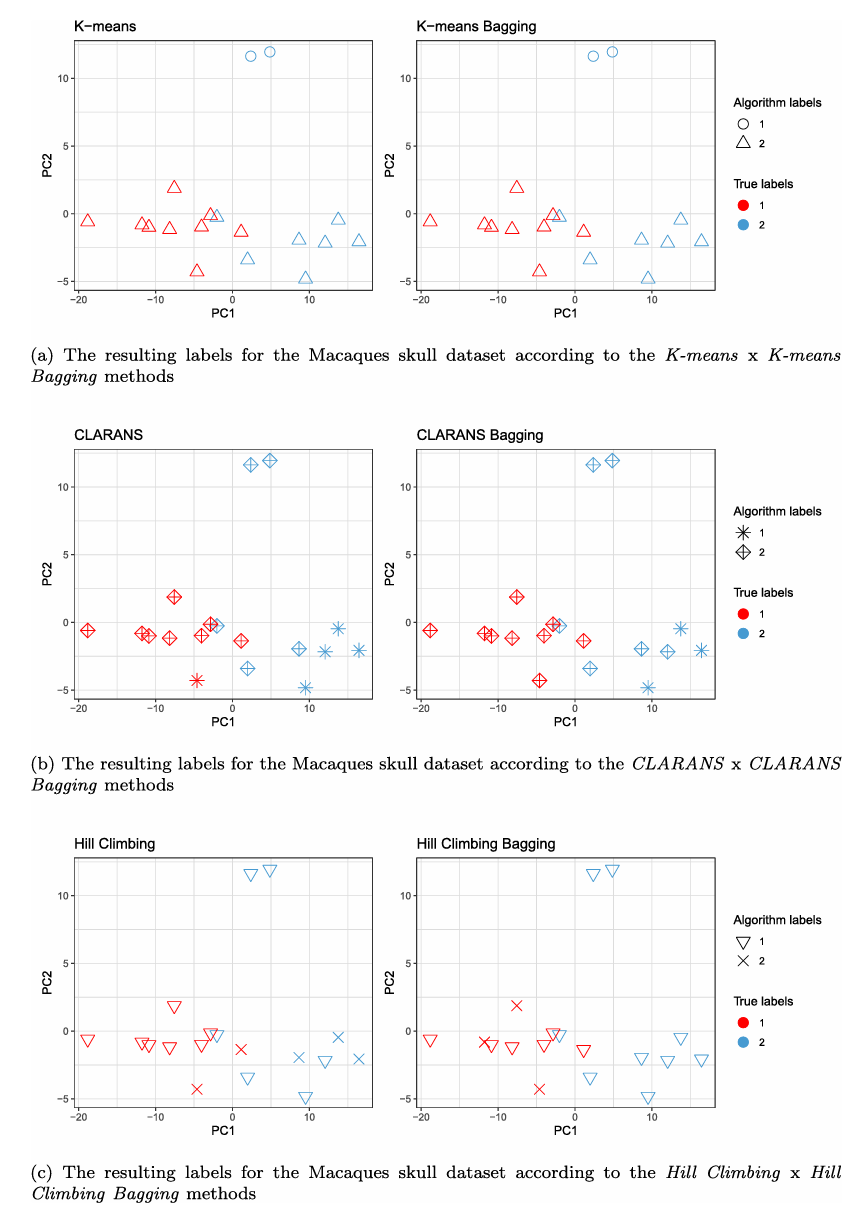
\includegraphics[height=0.66\textheight,keepaspectratio]{fig06_cluster_macacos.png}
    \vfill
    {\scriptsize Figura 6: Gráfico de dispersão dos agrupamentos para o conjunto de dados Crânio de Macaco.}
\end{frame}

\begin{frame}[shrink=10]
    \frametitle{Conjunto de dados 2: Cérebros humanos}
    \framesubtitle{$N=58$, $k=24$ marcos (12 por hemisfério)}

    \begin{columns}[c]
        \column{0.5\textwidth}
        \begin{itemize}
            \item $K=2$: 43 destros, 15 canhotos
            \item Todos os algoritmos melhoraram muito com Bagging.
            \item Ganhos expressivos no Rand Index e Fowlkes-Mallows Index.
        \end{itemize}
        \column{0.5\textwidth}
        \centering
        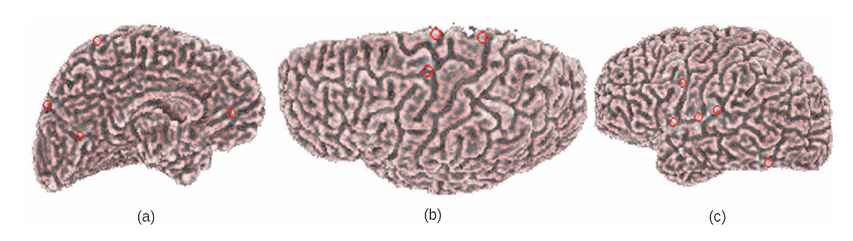
\includegraphics[width=0.8\linewidth,keepaspectratio]{fig07_landmarks_cerebro.png}
        \par {\scriptsize Figura 7: Visualização da localização de $k = 12$ marcos anatômicos do hemisfério esquerdo de um indivíduo.}
    \end{columns}
    
    \vspace{0.4cm}
    \centering
    \textbf{Tabela 8} (Nascimento et al., 2024): Resultados para o conjunto \textit{Brains}.\\[0.05cm]
    {\scriptsize Colunas \textit{relative}: ganho relativo (\%) para RI e FMI.}\\[0.1cm]
    \resizebox{0.95\linewidth}{!}{
        \begin{tabular}{@{}lcccccc@{}}
        \toprule
        Methods & \multicolumn{2}{c}{Rand index} & RI relative & \multicolumn{2}{c}{Fowlkes-mallows index} & FMI relative \\
        \cmidrule(lr){2-3} \cmidrule(lr){5-6}
         & Without bagging & B=100 & gain & Without bagging & B=100 & gain \\
        \midrule
        K-means & 0.5208 & 0.5783 & 11.03\% & 0.5882 & 0.6824 & 16.00\% \\
        CLARANS & 0.4967 & 0.5783 & 16.44\% & 0.5538 & 0.7282 & 31.13\% \\
        Hill Climbing & 0.4937 & 0.5783 & 17.15\% & 0.5452 & 0.7139 & 30.94\% \\
        \bottomrule
        \end{tabular}
    }
\end{frame}

\begin{frame}
    \frametitle{Cérebros: Agrupamento nas PCs}
    \framesubtitle{Benefício do Bagging em dados de maior complexidade}
    \centering
    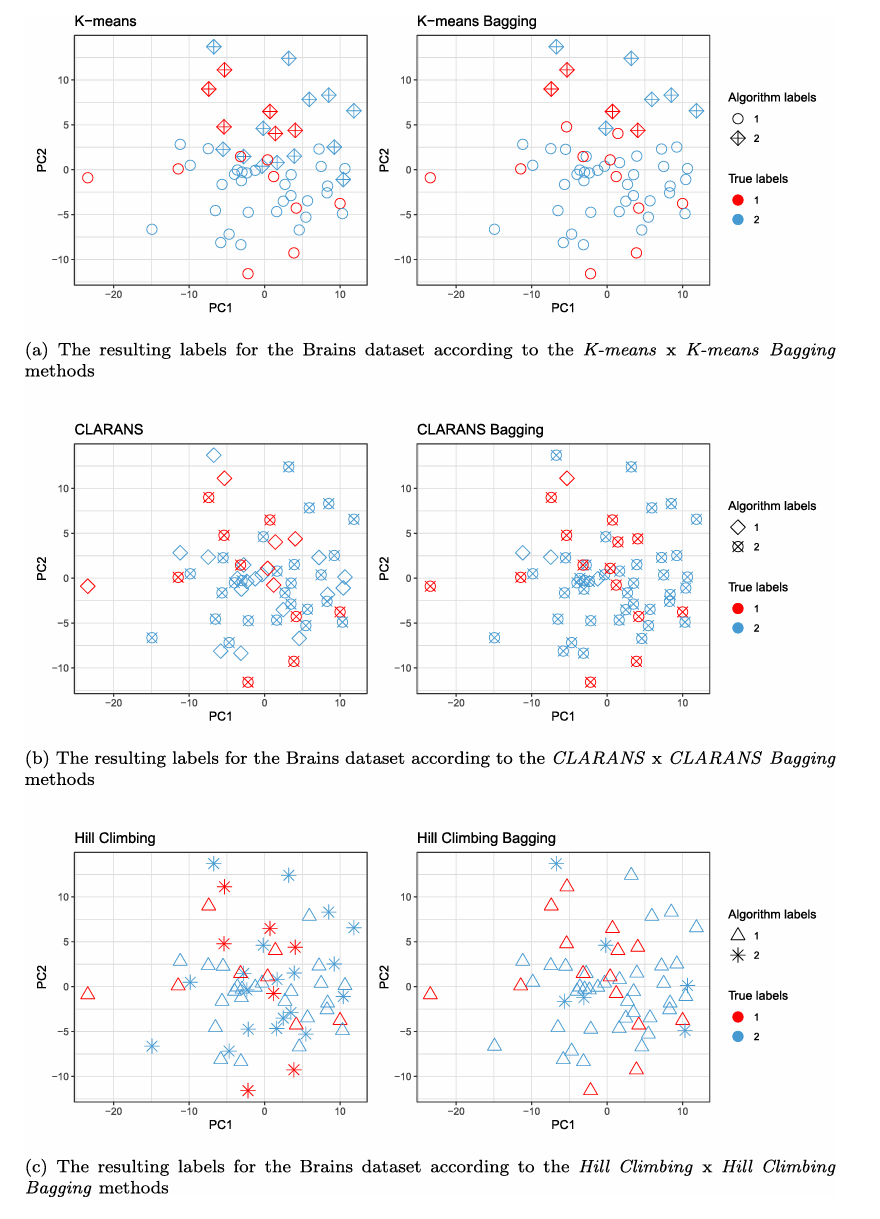
\includegraphics[height=0.66\textheight,keepaspectratio]{fig08_cluster_cerebros.png}
    \vfill
    {\scriptsize Figura 8: Gráfico de dispersão dos agrupamentos para o conjunto de dados Cérebros.}
\end{frame}

\section[Conclusões]{Conclusões e Trabalhos Futuros}

\begin{frame}
    \frametitle{Conclusões}
    \framesubtitle{Síntese dos resultados}

    \begin{block}{Síntese}
        Técnicas de \textbf{ensemble} (Bagging) melhoram a acurácia e a robustez do agrupamento de formas 3D, sobretudo em dados com \textbf{dispersão média ou alta} e em conjuntos maiores/complexos.
    \end{block}

    \begin{itemize}
        \item \textbf{CLARANS} e \textbf{Hill Climbing}: ganhos mais consistentes (simulação + Wilcoxon)
        \item \textbf{k-means}: melhorias limitadas na simulação; ganhos claros no conjunto \textit{Brains}
        \item Impacto prático: análises mais estáveis em morfometria médica e biológica
    \end{itemize}

    \begin{alertblock}{Custo computacional}
        Bagging exige $B=100$ execuções por algoritmo --- paralelização é direção natural.
    \end{alertblock}
\end{frame}

\begin{frame}
    \frametitle{Trabalhos Futuros}
    \framesubtitle{Extensões sugeridas pelos autores}

    \begin{enumerate}
        \item Explorar outros ensembles: \textbf{Boosting}, Random Subspace, Random Patches
        \item Comparar desempenho e custo com Bagging
        \item \textbf{Paralelização} e processamento distribuído das réplicas bootstrap
        \item Ampliar comparação de métodos de agrupamento 3D na literatura
    \end{enumerate}

    \vspace{0.5em}
    \begin{center}
        \Large Obrigado!\\
        \normalsize Perguntas?
    \end{center}
\end{frame}

\section[Refs]{Referências}

\begin{frame}[allowframebreaks]
    \frametitle{Referências Principais}
    \footnotesize
    \begin{thebibliography}{99}
        \bibitem{nascimento2024}
        Nascimento, I.; Ospina, R.; Amorim, G.
        Using Bagging to improve clustering methods in the context of three-dimensional shapes.
        \textit{Advances in Data Analysis and Classification}, 2024.
        \url{https://doi.org/10.1007/s11634-024-00602-9}

        \bibitem{dryden2016}
        Dryden, I.\ L.; Mardia, K.\ V.
        \textit{Statistical Shape Analysis: With Applications in R}, 2nd ed.
        Wiley, 2016.

        \bibitem{vinue2014}
        Vinué, G.; Simó, A.; Alemany, S.
        The K-means algorithm for 3D shapes with an application to apparel design.
        \textit{Advances in Data Analysis and Classification}, 10(1):103--132, 2014.

        \bibitem{breiman1996}
        Breiman, L.
        Bagging predictors.
        \textit{Machine Learning}, 24(2):123--140, 1996.

        \bibitem{dudoit2003}
        Dudoit, S.; Fridlyand, J.
        Bagging to improve the accuracy of a clustering procedure.
        \textit{Bioinformatics}, 19(9):1090--1099, 2003.

        \bibitem{ng2002}
        Ng, R.\ T.; Han, J.
        CLARANS: A method for clustering objects for spatial data mining.
        \textit{IEEE Transactions on Knowledge and Data Engineering}, 14(5):1003--1016, 2002.

        \bibitem{kendall1984}
        Kendall, D.\ G.
        Shape manifolds, procrustean metrics, and complex projective spaces.
        \textit{Bulletin of the London Mathematical Society}, 16(2):81--121, 1984.

        \bibitem{assis2021}
        Assis, E.\ C.\ D.; Souza, R.\ M.\ C.\ R.\ D.; Amaral, G.\ J.\ A.\ D.
        Using bagging to enhance clustering procedures for planar shapes.
        \textit{International Journal of Business Intelligence and Data Mining}, 18(1):30--48, 2021.
    \end{thebibliography}
\end{frame}


\end{document}

